% =============================================================================
%  Dinamica3_Fase2_Diapositiva1.tex — Dinámica 3, Fase 2, Diapositiva 1:
%  lectura normal / estímulo confuso. Texto intercalado del cap. 34 de
%  Rayuela tal como está impreso (líneas impares: novela; pares: Oliveira).
%  Fuente: Cortázar, Rayuela, Alfaguara, p. 212, líneas 1–16.
%  Formato 16:9. Compilar con: bash ../../../compilar_diapositivas.sh
% =============================================================================
\documentclass[tikz,border=0pt]{standalone}
\usepackage[utf8]{inputenc}
\usepackage[T1]{fontenc}
\usepackage{ebgaramond}

% ── Parámetros ────────────────────────────────────────────────────────────────
\def\TamLetra{20}       % tamaño de letra, en pt
\def\Interlinea{27.5}   % interlineado, en pt

% ── Paleta (pergamino de la Fase 1) ───────────────────────────────────────────
\definecolor{Pergamino}{HTML}{F1EBDD}
\definecolor{PergaminoBorde}{HTML}{DCCFB4}
\definecolor{Fibra}{HTML}{B9A27A}
\definecolor{Tinta}{HTML}{2B2620}
\definecolor{Referencia}{HTML}{6B5A43}

% ── Dimensiones (16:9) ────────────────────────────────────────────────────────
\def\ancho{32}
\def\alto{18}

\begin{document}
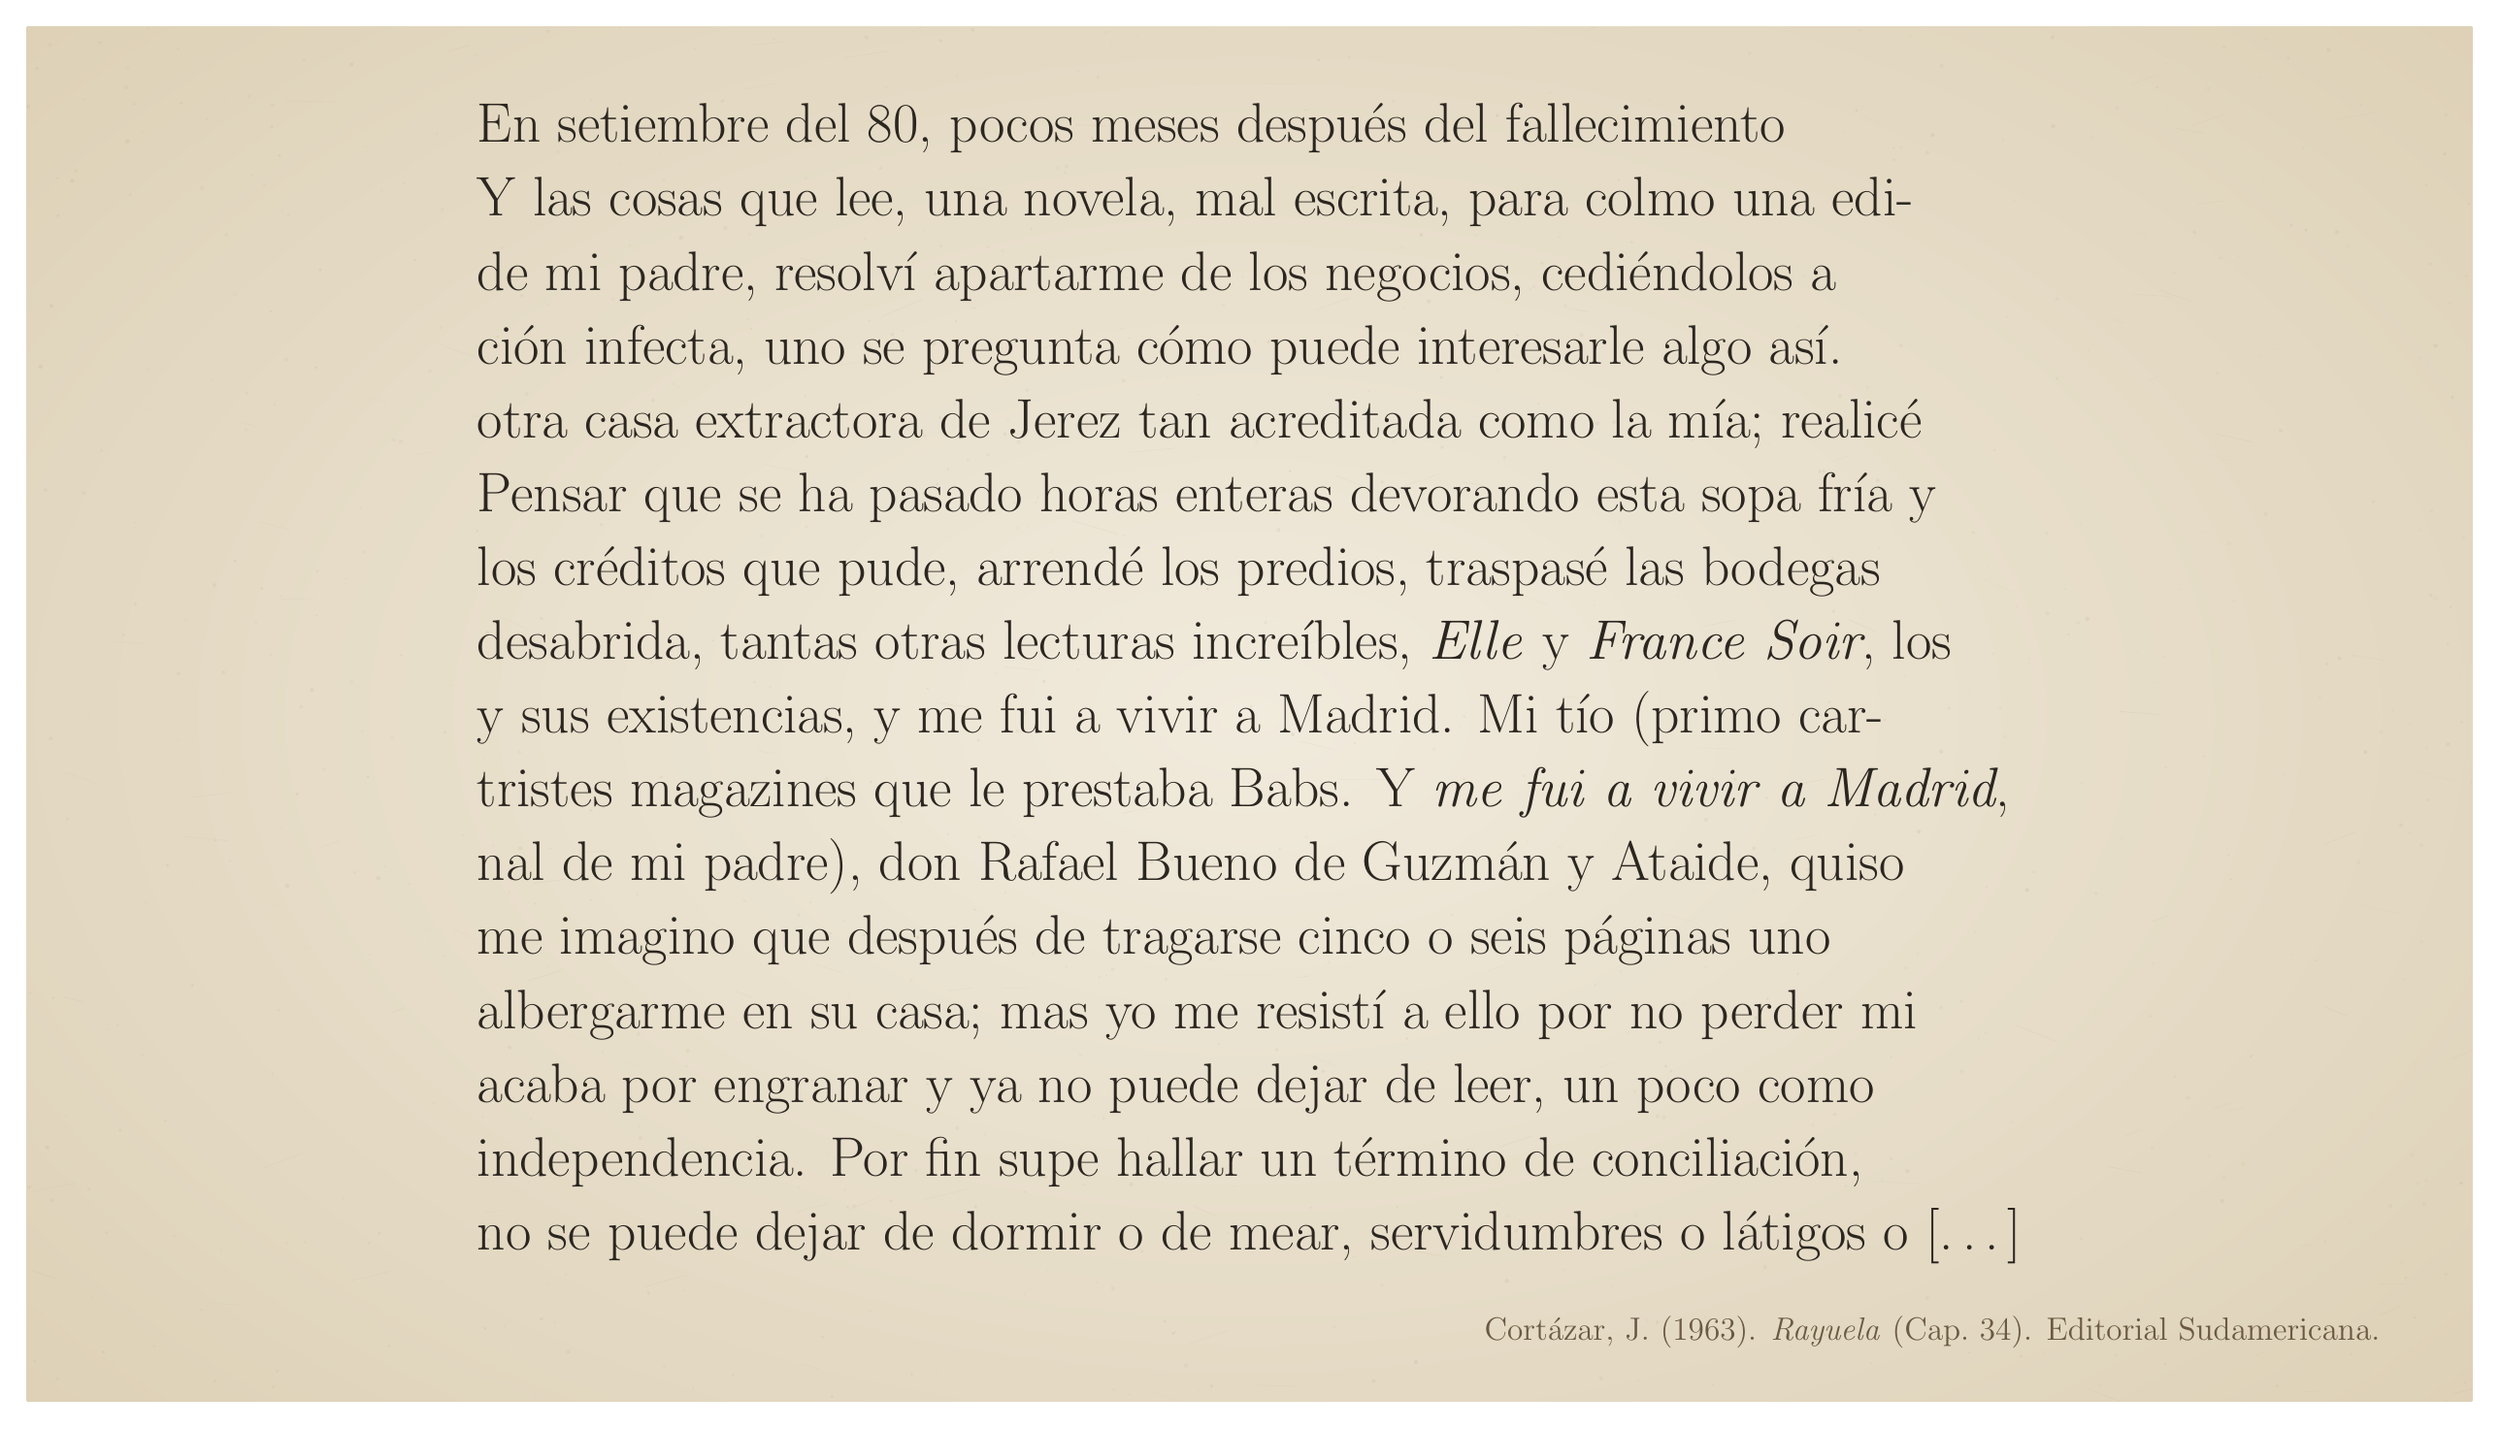
\begin{tikzpicture}
  \useasboundingbox (0,0) rectangle (\ancho,\alto);
  \clip (0,0) rectangle (\ancho,\alto);

  % Fondo con viñeta
  \fill[PergaminoBorde] (0,0) rectangle (\ancho,\alto);
  \shade[inner color=Pergamino, outer color=PergaminoBorde]
    (\ancho/2,\alto/2) ellipse [x radius=0.72*\ancho, y radius=0.80*\alto];

  % Textura (misma semilla que la Fase 1)
  \pgfmathsetseed{1914}
  \foreach \i in {1,...,900}{
    \pgfmathsetmacro{\x}{rnd*\ancho}
    \pgfmathsetmacro{\y}{rnd*\alto}
    \pgfmathsetmacro{\r}{0.008+0.02*rnd}
    \pgfmathsetmacro{\o}{0.05+0.12*rnd}
    \fill[Fibra, opacity=\o] (\x,\y) circle (\r);
  }
  \foreach \i in {1,...,140}{
    \pgfmathsetmacro{\x}{rnd*\ancho}
    \pgfmathsetmacro{\y}{rnd*\alto}
    \pgfmathsetmacro{\l}{0.15+0.5*rnd}
    \pgfmathsetmacro{\a}{-25+50*rnd}
    \pgfmathsetmacro{\o}{0.04+0.08*rnd}
    \draw[Fibra, opacity=\o, line width=0.25pt, rotate around={\a:(\x,\y)}]
      (\x,\y) -- ++(\l,0);
  }

  % Texto intercalado, con los cortes de línea del libro
  \node[text=Tinta, align=left, inner sep=0pt,
        font=\fontsize{\TamLetra}{\Interlinea}\selectfont]
    at (\ancho/2,\alto/2+0.4) {%
      En setiembre del 80, pocos meses después del fallecimiento\\
      Y las cosas que lee, una novela, mal escrita, para colmo una edi-\\
      de mi padre, resolví apartarme de los negocios, cediéndolos a\\
      ción infecta, uno se pregunta cómo puede interesarle algo así.\\
      otra casa extractora de Jerez tan acreditada como la mía; realicé\\
      Pensar que se ha pasado horas enteras devorando esta sopa fría y\\
      los créditos que pude, arrendé los predios, traspasé las bodegas\\
      desabrida, tantas otras lecturas increíbles, \textit{Elle} y \textit{France Soir}, los\\
      y sus existencias, y me fui a vivir a Madrid. Mi tío (primo car-\\
      tristes magazines que le prestaba Babs. Y \textit{me fui a vivir a Madrid},\\
      nal de mi padre), don Rafael Bueno de Guzmán y Ataide, quiso\\
      me imagino que después de tragarse cinco o seis páginas uno\\
      albergarme en su casa; mas yo me resistí a ello por no perder mi\\
      acaba por engranar y ya no puede dejar de leer, un poco como\\
      independencia. Por fin supe hallar un término de conciliación,\\
      no se puede dejar de dormir o de mear, servidumbres o látigos o […]%
    };

  % Referencia APA
  \node[anchor=south east, text=Referencia, inner sep=0pt,
        font=\fontsize{13}{16}\selectfont]
    at (\ancho-1.2,0.7)
    {Cortázar, J. (1963). \textit{Rayuela} (Cap.~34). Editorial Sudamericana.};
\end{tikzpicture}
\end{document}
